\documentclass[12pt]{article}
\usepackage[utf8]{inputenc}
\usepackage{amsmath}
\usepackage{graphicx}
\usepackage{hyperref}
\usepackage{geometry}
\geometry{margin=1in}

\title{Algorithms: Design and Analysis \\ Final Report}
\author{
  Team 53 \\
  Members: Qurba Mushtaq 08232, Hiba Shahid 08036
}
\date{}

\begin{document}

\maketitle

\noindent\textbf{Reviewed research paper title:} \\
\textit{Bidirectional Dijkstra's Algorithm is Instance-Optimal} \\
by Bernhad Haeupler, Richard Hladik, Vaclav Rozhon, Robert E. Tarjan

% \vspace{1em}
% \noindent\textbf{GitHub:} 
% \url{https://github.com/HibaShahidA/Bidirectional-Dijkstra}

\section{Introduction-Problem and Contribution}
For any given graphs, the algorithm with the near-optimal time complexity for finding the shortest $st$-path is Dijkstra's algorithm. However, for much larger graphs, as seen in real world scenarios, there are other algorithms that perform far better. One of these algorithms is bidirectional search using the Dijkstra's algorithm. The way it is performed is through executing Dijkstra's algorithm from both endpoints ($s$ and $t$) in parallel. 

In huge graphs, specifically (non-negative) weighted multigraphs - both directed and undirected - use of bidirectional search is instance-optimal with respect to the number of edges it explores. This is different from the general Dijkstra's algorithm that is executed by traversing through all paths to find the shortest one - exploring the entire input graph. 

Although the worst-case complexity remains the same, bidirectional search has an upper hand on the Dijkstra's algorithm - especially for unweighted graphs where it is instance-optimal up to a factor of O(delta) where delta is the maximum degree of the graph.


\section{Algorithm Design, Correctness, and Optimality}

\subsection{Unidirectional vs. Bidirectional Dijkstra}
The paper proves that unidirectional Dijkstra is instance-optimal under a restricted setting where only out-neighbor access is allowed. In such a model, even randomized algorithms cannot outperform it.

The proposed bidirectional algorithm runs two Dijkstra searches—one from the source ($s$) and one from the target ($t$)—alternating between them. At each step, it relaxes one edge from the active frontier. The search stops when:
\[
\hat{d}(s,u_s) + \hat{d}(u_t, t) > \mu
\]
where \( \mu \) is the shortest path length found so far.
\[
\mu = \min_{v \in S_f \cap S_b}(d_f(v) + d_b(v))
\]
and $\hat{d}(s,u_s)$ is the distance from the source to the current forwards node, while $\hat{d}(u_t, t)$ is the distance from the current backward node to the sink. This ensures no better path remains undiscovered. This is explained in further detail in our implementation in section \ref{sec:algo}.

For the sake of visualizing and understanding, think of two people walking towards one another along the shortest - one from the source and one from the target. If both take the optimal steps and meet in the middle, neither has to walk the full path. Similarly, in the bidirectional search, the search path does not have to explore the entire input graph. 

\begin{figure}[h]
\centering
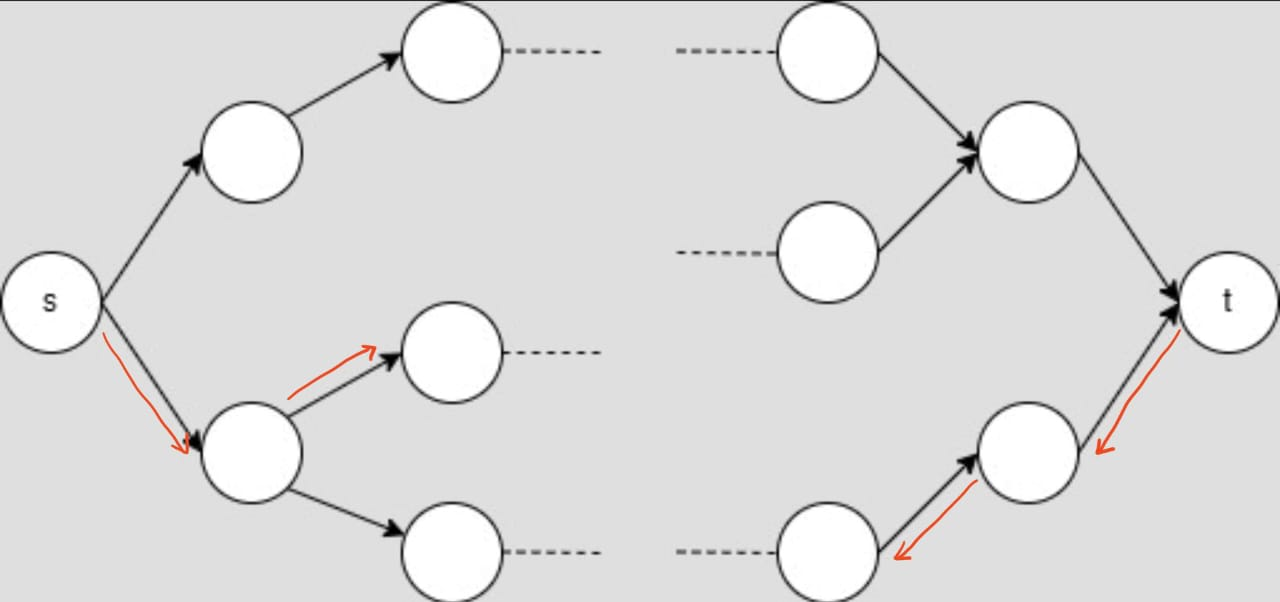
\includegraphics[width=0.8\textwidth]{BidirectionalDijkstra-cp2-edit.jpg}
\caption{The \textbf{red arrows} show the traversal that the algorithm takes. Irrespective of the direction of the edges, since the reverse traversal works similar to that of the forward traversal (much like residual graph traversal).}
\end{figure}

\subsection{Correctness and Comparison}
Once the forward and backward searches meet at a common vertex or edge, the path is built by merging the two. If any shorter path existed, it would have been found before the stopping condition was satisfied. This guarantees correctness.

While Dijkstra explores more edges than necessary and A* requires extra heuristic information, the bidirectional version in this paper achieves strong performance without such assumptions. Even in large graphs, it explores fewer edges and runs faster in practice.

\subsection{Instance Optimality}
To prove that no correct algorithm can consistently outperform it, the authors construct two graph versions \( G \) and \( G' \). An algorithm that skips a critical edge in \( G \) will return an incorrect result in \( G' \), where that edge is essential. This contradiction shows that the bidirectional algorithm explores the fewest possible edges without compromising correctness.

\noindent\textbf{Input:} The input of the algorithm is a graph \( G = (V, E) \) with non-negative edge weights, a source vertex \( s \) and a target vertex \( t \). \\
\textbf{Output:} The length and path of the shortest path from \( s \) to \( t \), if a path exists. \( \infty \) otherwise.

The input graph \( G \), each with a source vertex \( s \) and a target vertex \( t \), is traversed such that an optimal path search is started from \( s \) and an optimal path search is started from \( t \) simultaneously. Once the traversal from both endpoints meets, it is terminated - a path has been found.

\section{Comparison}
The paper proves that Bidirectional Dijkstra's algorithm is instance-optimal (mathematically optimal for every individual input graph, not just in worst-case scenarios) for finding shortest paths in weighted graphs, meaning no correct algorithm can outperform it by more than a constant factor on any input. Unlike standard Dijkstra's algorithm, which explores outward from the source, bidirectional search runs two simultaneous Dijkstra executions (forward from s and backward from t).

Previous variants (Dantzig, Nicholson, Pohl) lacked instance-optimality guarantees due to two key flaws:

Their selection rules ("None of those approaches [Dantzig's alternation, Nicholson's closest-node, Pohl's queue-size] achieve the instance-optimality guarantees" - Theorem 1)

Their stopping conditions (Early versions used "a seemingly natural stopping condition that is not correct" - stopping at first intersection rather than path confirmation)

This work overcomes these limitations by introducing:

A strict alternation rule (one forward step, one backward step)

A correct stopping condition (ensures termination only when the shortest path is confirmed)

The result holds for both directed and undirected graphs with positive weights, while in unweighted graphs, the algorithm is optimal up to a factor of \( O(\Delta) \) (scales with the graph's maximum degree \( \Delta \)). Unlike A* (a heuristic-guided search that uses estimated distances to prioritize nodes), which relies on heuristics (problem-specific estimates to guide search), bidirectional Dijkstra is optimal without additional information, making it the best general-purpose shortest-path algorithm in this setting.

\section{Implementation Strategy}

\subsection{How It Works}
\label{sec:algo}
The bidirectional Dijkstra algorithm works by running two simultaneous searches—one from the source node \( s \) and one from the target node \( t \). Each search maintains its own set of distances and predecessors.

\begin{itemize}
    \item \textbf{Forward Search:} Begins at node \( s \), using a priority queue to explore vertices. It updates shortest distances (\texttt{d\_forward}) and predecessors (\texttt{pred\_forward}) as it goes.
    
    \item \textbf{Backward Search:} Begins at node \( t \), exploring the graph in reverse (i.e., following incoming edges in directed graphs). It updates \texttt{d\_backward} and \texttt{pred\_backward}.

    \item \textbf{Meeting Point:} The forward and backward searches eventually meet at a common vertex or edge. This meeting point is used to construct a complete path from \( s \) to \( t \).

    \item \textbf{Stopping Condition:} The algorithm stops when the combined current distances from both searches exceed the best known path length (\( \mu \)). This ensures that continuing would not find a better path.

    \item \textbf{Path Construction:} Once the searches meet, the path is built by combining the forward path to the meeting point with the backward path from that point to \( t \). The final result is the shortest path from \( s \) to \( t \).
\end{itemize}

\subsection{Correctness Testing}
To ensure the implementation was correct, we tested it on graphs of varying sizes and edge densities. Sample test cases included:
\begin{itemize}
    \item Small graphs where shortest paths could be calculated manually.
    \item Graphs with multiple shortest paths of the same length.
    \item Disconnected graphs to ensure no invalid paths were returned.
\end{itemize}

In each case, the paths and distances returned matched those from standard Dijkstra and NetworkX’s implementation. We also utilized a custom $Graph$ class to emulate different types of graphs. On a separate note, we also tried and tested the algorithm on different types of graphs, including: expanding graphs, Chung Lu graphs, power law graphs, and hyperbolic graphs.

\subsection{Challenges and Enhancements}
The main challenge was implementing the correct stopping condition. In early tests, the algorithm stopped too early or too late, depending on how we computed the current best path length $\mu$. We fixed this by tracking the shortest overlapping path during exploration and applying the correct check condition.

We enhanced our code to collect the number of edge relaxations and average execution time for each algorithm over multiple iterations. This allowed us to generate meaningful visual comparisons and see how performance scaled with graph size. We also generated synthetic graphs of different types using a helper function and NetworkX’s random graph generators.

We aimed to record the the trends of applying the algorithm on larger and more complex graphs, and we managed to record the performance through the terminal, and it was successful, as proposed by the paper. However, due to the limited processor power we had, we decided not to delve much into the complex graphs, and remain focused on directed weighted, undirected weighted, and unweighted graphs as per the focus of the paper.

\section{Empirical Verification}
To prove that the proposed algorithm is, in fact, instance-optimal, we evaluated its performance on varying graphs and compared it against classical Dijkstra and A*. We focused on two metrics: \textbf{execution time} and \textbf{number of edges traversed}. \\[1ex]

\begin{figure}[h]
    \centering
    \includegraphics[width=0.75\textwidth]{comparison_times.png}
    \caption{Comparison of Execution Time across Algorithms}
    \label{fig:exec-time}
\end{figure}

\begin{figure}[h]
    \centering
    \includegraphics[width=0.75\textwidth]{comparison_edges.png}
    \caption{Comparison of Edges Traversed across Algorithms}
    \label{fig:edges-traversed}
\end{figure}

\break
From the figures \ref{fig:exec-time} and \ref{fig:edges-traversed}, it is evident that the bidirectional Dijkstra algorithm outperforms traditional Dijkstra and A* in the no-heuristic setting. This difference becomes especially clear in larger graphs. The number of edges it explores is much lower, and this leads to shorter execution times as well. This supports the paper’s claim that bidirectional Dijkstra is instance-optimal.

\section{Complexity Analysis}
The time and space complexity of Bidirectional Dijkstra’s algorithm depends on the number of vertices \( V \) and edges \( E \) in the graph.

In the worst case, the algorithm behaves similarly to standard Dijkstra's algorithm:
\begin{itemize}
    \item Time complexity: \( O((V + E) \log V) \), assuming a binary heap is used for the priority queue.
    \item Space complexity: \( O(V + E) \), due to storing distances, predecessors, and the graph structure.
\end{itemize}

However, in practice, the bidirectional approach explores far fewer nodes and edges, especially in large graphs. Since the searches start from both ends, the area explored is roughly half in each direction. This leads to a practical improvement in performance, though the theoretical worst-case remains similar. This is evident in the trends we monitored in figures \ref{fig:exec-time} and \ref{fig:edges-traversed}.

In graphs with small diameters or dense connections, the benefits of bidirectional search are even more noticeable. Our empirical results confirm that the average number of edge relaxations and execution time are significantly lower than unidirectional Dijkstra.

\section{Datasets and Testing Material}
We tested the algorithm on both manually constructed graphs and synthetic data. The larger test cases were generated using our own functions and \textbf{NetworkX}’s random graph tools. Each algorithm was run multiple times on the same inputs, and average times and edge counts were recorded.

\section{Future Work and Reflections}
It would be interesting to see if these instance-optimality ideas can be extended to A* or other heuristic-based algorithms. Another idea is testing the algorithm on real-world graphs like road networks or social graphs to see if the observed gains carry over. We are also curious about how the results would differ on undirected graphs or graphs with zero-weight edges.

\section{GitHub repository}
\textbf{URL:} \url{https://github.com/HibaShahidA/Bidirectional-Dijkstra}

\end{document}
